\chapter{Semi-parametric and non-parametric models}\label{chap11}

\section*{Solutions of Exercises}\label{sec11_1}
\begin{enumerate}[leftmargin=*]

\item Simulate a semi-parametric regression where  
\begin{align*}
	y_i &= 0.5x_{i1} - 1.2x_{i2} + \mu_i, \\
	p(\mu_i) &= 
	0.3 \phi(\mu_i \mid -0.5,0.5^2) + 0.7 \phi(\mu_i \mid 1,0.8^2).		
\end{align*}
Assume that $x_{i1}$ and $x_{i2}$ follow a standard normal distribution and that the sample size is 1,000. Perform inference in this model assuming that the number of components is unknown. Start with $H=5$ and use non-informative priors, setting $\alpha_{h0}=\delta_{h0}=0.01$, $\bm{\beta}_0=\bm{0}_2$, $\bm{B}_0=\bm{I}_2$, $\mu_{h0}=0$, $\sigma^2_{\mu 0}=10$, and $\bm{\alpha}_0=[1/H \ \dots \ 1/H]^{\top}$. Use 6,000 MCMC iterations, a burn-in period of 4,000, and a thinning parameter of 2. Compare the population parameters with the posterior estimates and plot the population density along with the posterior density estimate of $\bm{\mu}$ (the mean, and the 95\% credible interval).\\

\textbf{Answer}

We can see from the posterior estimates that three components disappear after the burn-in iterations. The 95\% credible intervals encompass the population values of all parameters, and the posterior density estimate closely matches the population density. See Figure \ref{figPMPDens}, where the black line represents the population density, the blue line denotes the posterior mean density estimate, and the shaded light blue area corresponds to the 95\% credible interval.
 
\begin{tcolorbox}[enhanced,width=4.67in,center upper,
	fontupper=\large\bfseries,drop shadow southwest,sharp corners]
	\textit{R code. Simulation: Semi-parametric Gaussian mixture}
	\begin{VF}
		\begin{lstlisting}[language=R]
rm(list = ls()); set.seed(010101)
# Simulate data from a 2-component mixture model
n <- 1000
x1 <- rnorm(n); x2 <- rnorm(n)
B <- c(0.5, -1.2); X <- cbind(x1, x2)
z <- rbinom(n, 1, 0.3)  # Latent class indicator
mu <- ifelse(z == 0, rnorm(n, -0.5, 0.5), rnorm(n, 1, 0.8))
plot(density(mu))
y <- X%*%B + mu
# Hyperparameters
d0 <- 0.001; a0 <- 0.001
b0 <- rep(0, 2); B0 <- diag(2); B0i <- solve(B0)
mu0 <- 0; sig2mu0 <- 10
H <- 5; a0h <- rep(1/H, H)
# MCMC parameters
mcmc <- 2000
burnin <- 4000
tot <- mcmc + burnin
thin <- 2
# Gibbs sampling functions
PostSig2 <- function(Beta, muh, Xh, yh){
	Nh <- length(yh)
	an <- a0 + Nh
	dn <- d0 + t(yh - muh - Xh%*%Beta)%*%(yh - muh - Xh%*%Beta)
	sig2 <- invgamma::rinvgamma(1, shape = an/2, rate = dn/2)
	return(sig2)
}
PostBeta <- function(sig2, mu, X, y, Psi){
	XtX <- matrix(0, 2, 2)
	Xty <- matrix(0, 2, 1)
	Hs <- length(mu)
	for(h in 1:Hs){
		idh <- which(Psi == h)
		if(length(idh) == 1){
			Xh <- matrix(X[idh,], 1, 2)
			XtXh <- sig2[h]^(-1)*t(Xh)%*%Xh
			yh <- y[idh]
			Xtyh <- sig2[h]^(-1)*t(Xh)%*%(yh - mu[h])
		}else{
			Xh <- X[idh,]
			XtXh <- sig2[h]^(-1)*t(Xh)%*%Xh
			yh <- y[idh]
			Xtyh <- sig2[h]^(-1)*t(Xh)%*%(yh - mu[h])
		}
		XtX <- XtX + XtXh
		Xty <- Xty + Xtyh
	}
	Bn <- solve(B0i + XtX)
	bn <- Bn%*%(B0i%*%b0 + Xty)
	Beta <- MASS::mvrnorm(1, bn, Bn)
	return(Beta)
}
\end{lstlisting}
	\end{VF}
\end{tcolorbox} 

\begin{tcolorbox}[enhanced,width=4.67in,center upper,
	fontupper=\large\bfseries,drop shadow southwest,sharp corners]
	\textit{R code. Simulation: Semi-parametric Gaussian mixture}
	\begin{VF}
		\begin{lstlisting}[language=R]
Postmu <- function(sig2h, Beta, Xh, yh){
	Nh <- length(yh)
	sig2mu <- (1/sig2mu0 + Nh/sig2h)^(-1)
	mun <- sig2mu*(mu0/sig2mu0 + sum((yh - Xh%*%Beta))/sig2h)
	mu <- rnorm(1, mun, sig2mu^0.5)
	return(mu)
}
PostBetas <- matrix(0, mcmc+burnin, 2)
PostPsi <- matrix(0, mcmc+burnin, n)
PostSigma2 <- list(); PostMu <- list()
PostLambda <- list(); Reg <- lm(y ~ X)
Beta <- Reg$coefficients[2:3]; Res <- Reg$residuals
plot(density(Res))
Resq <- quantile(Res, c(0.2, 0.4, 0.6, 0.8))
Id1 <- which(Res <= Resq[1])
Id2 <- which(Res > Resq[1] & Res <= Resq[2])
Id3 <- which(Res > Resq[2] & Res <= Resq[3])
Id4 <- which(Res > Resq[3] & Res <= Resq[4])
Id5 <- which(Res > Resq[4])
Nh <- rep(n/H, H); Lambda <- rep(1/H, H)
MU <- c(mean(Res[Id1]), mean(Res[Id2]), mean(Res[Id3]), mean(Res[Id4]), mean(Res[Id5]))
Sig2 <- c(var(Res[Id1]), var(Res[Id2]), var(Res[Id3]), var(Res[Id4]), var(Res[Id5]))
Psi <- rep(NA, n); Hs <- length(MU)
pb <- winProgressBar(title = "progress bar", min = 0, max = tot, width = 300)
for(s in 1:tot){
	for(i in 1:n){
		lambdai <- NULL
		for(h in 1:Hs){
			lambdaih <- Lambda[h]*dnorm(y[i] - X[i,]%*%Beta, MU[h], Sig2[h]^0.5)
			lambdai <- c(lambdai, lambdaih)
		}
		Psi[i] <- sample(1:Hs, 1, prob = lambdai)
	}
	PostPsi[s, ] <- Psi
	Hs <- length(table(Psi))
	for(h in 1:Hs){
		idh <- which(Psi == h)
		Sig2[h] <- PostSig2(Beta = Beta, muh = MU[h], Xh = X[idh,], yh = y[idh])
		MU[h] <- Postmu(sig2h = Sig2[h], Beta = Beta, Xh = X[idh,], yh = y[idh])
	}
	PostSigma2[[s]] <- Sig2
	PostMu[[s]] <- MU 
	Beta <- PostBeta(sig2 = Sig2, mu = MU, X = X, y = y, Psi = Psi)
	PostBetas[s,] <- Beta
	Lambda <- sort(MCMCpack::rdirichlet(1, a0h[1:Hs] + table(Psi)), decreasing = TRUE)
	PostLambda[[s]] <- Lambda
	setWinProgressBar(pb, s, title=paste( round(s/tot*100, 0),"% done"))
}
close(pb)
\end{lstlisting}
	\end{VF}
\end{tcolorbox}

\begin{tcolorbox}[enhanced,width=4.67in,center upper,
	fontupper=\large\bfseries,drop shadow southwest,sharp corners]
	\textit{R code. Simulation: Semi-parametric Gaussian mixture}
	\begin{VF}
		\begin{lstlisting}[language=R]
keep <- seq(burnin, tot, thin)
PosteriorBetas <- coda::mcmc(PostBetas[keep,])
summary(PosteriorBetas); plot(PosteriorBetas)
PosteriorPsi <- PostPsi[keep,]
Clusters <- sapply(1:length(keep), function(i){length(table(PosteriorPsi[i,]))})
PosteriorSIGMA <- matrix(NA, length(keep), 2)
PosteriorMU <- matrix(NA, length(keep), 2)
PosteriorLAMBDA <- matrix(NA, length(keep), 2)
l <- 1
for (s in keep){
	PosteriorSIGMA[l,] <- PostSigma2[[s]][1:2]
	PosteriorMU[l,] <- PostMu[[s]][1:2]
	PosteriorLAMBDA[l,] <- PostLambda[[s]][1:2]
	l <- l + 1
}
summary(coda::mcmc(PosteriorSIGMA))
summary(coda::mcmc(PosteriorMU))
summary(coda::mcmc(PosteriorLAMBDA))
mus <- seq(-3, 4, 0.01)
DensityEst <- function(par, eval){
	lambda1 <- par[1]; lambda2 <- par[2]
	mu1 <- par[3]; mu2 <- par[4]
	sd1 <- par[5]; sd2 <- par[6]
	Dens <- lambda1 * dnorm(eval, mu1, sd1) + lambda2 * dnorm(eval, mu2, sd2)
	return(Dens)
}
par <- cbind(PosteriorLAMBDA, PosteriorMU, PosteriorSIGMA^0.5)
DensEval <- matrix(NA, length(keep), length(mus))
DensPop <- rep(NA, length(mus))
for(r in 1:length(mus)){
	for(l in 1:length(keep)){
		DensEval[l, r] <- DensityEst(par = par[l,], eval = mus[r])
	}
	DensPop[r] <- DensityEst(par = c(0.7, 0.3, -0.5, 1, 0.5, 0.8), eval = mus[r]) 
}
library(dplyr); library(ggplot2); require(latex2exp)
DataDens <- tibble(t = mus, Pop = DensPop, lower = apply(DensEval, 2, quantile, probs = 0.025), upper = apply(DensEval, 2, quantile, probs = 0.975), meanT = colMeans(DensEval))
plot_filtering_estimates <- function(df) {
	p <- ggplot(data = df, aes(x = t)) + 	geom_ribbon(aes(ymin = lower, ymax = upper), alpha = 1, fill = "lightblue") + 	geom_line(aes(y = Pop, color = "True Value"), linewidth = 0.5) + 	geom_line(aes(y = meanT, color = "Estimate"), linewidth = 0.5) +
	scale_color_manual(values = c("True Value" = "black", "Estimate" = "blue")) + xlab(TeX("$\\mu$")) + ylab("Density") + 	labs(title = "Density: Stochastic Errors", color = "") + theme_minimal()
	print(p)
}
plot_filtering_estimates(DataDens)
\end{lstlisting}
	\end{VF}
\end{tcolorbox}

\begin{figure}[!h]
	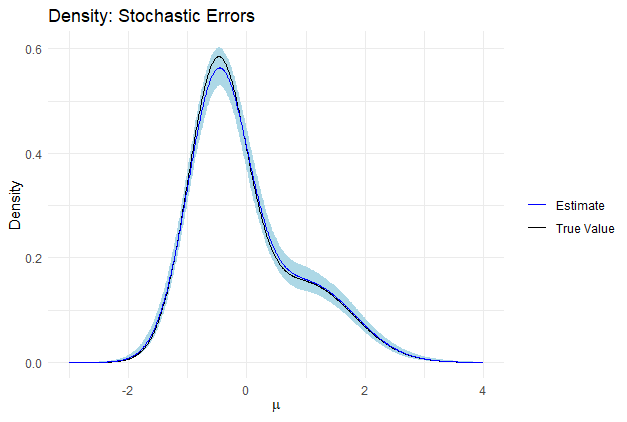
\includegraphics[width=340pt, height=200pt]{Chapters/chapter11/figures/DensEstSE.png}
	\caption[List of figure caption goes here]{Posterior density estimate: Stochastic errors.}\label{figPMPDens}
\end{figure}

\item Use the dataset \textit{MarijuanaColombia.csv} from our GitHub repository to perform inference on the demand for marijuana in Colombia. This dataset contains information on the (log) monthly demand in 2019 from the National Survey of the Consumption of Psychoactive Substances. It includes variables such as the presence of a drug dealer in the neighborhood (\textit{Dealer}), gender (\textit{Female}), indicators of good physical and mental health (\textit{PhysicalHealthGood} and \textit{MentalHealthGood}), age (\textit{Age} and \textit{Age2}), years of schooling (\textit{YearsEducation}), and (log) prices of marijuana, cocaine, and crack by individual (\textit{LogPriceMarijuana}, \textit{LogPriceCocaine}, and \textit{LogPriceCrack}). The sample size is 1,156.

Estimate a finite Gaussian mixture regression using non-informative priors, that is, $\alpha_{0}=\delta_{0}=0.01$, $\boldsymbol{\beta}_{0}=\boldsymbol{0}_K$, $\boldsymbol{B}_{0}=\boldsymbol{I}_K$, and and $\boldsymbol{\alpha}_0=[1/H \ \dots \ 1/H]^{\top}$, $K$ is the number of regressors, 11 including the intercept. The number of MCMC iterations is 5,000, the burn-in is 1,000, and the thinning parameter is 2. Start with five potential clusters. Obtain the posterior distribution of the own-price elasticity of marijuana and the cross-price elasticities of marijuana demand with respect to the prices of cocaine and crack.\\

\textbf{Answer:}

The following code demonstrates how to perform inference in this model. The results indicate the presence of four clusters, with mean probabilities of 0.64, 0.14, 0.12 and 0.10, and 95\% credible intervals of (0.60, 0.67), (0.12,0.16), (0.10,0.14) and (0.08, 0.12), respectively.  

The 95\% posterior credible interval for the own-price elasticities of the most representative group, which comprises two-thirds of the sample, is $(-0.55, -0.26)$. Additionally, the 95\% credible interval for the cross-price elasticities with respect to cocaine is $(0.01, 0.35)$, while that with respect to crack is $(0.07, 0.43)$.

These results suggest that marijuana is an inelastic good for these individuals and that there is substitution between marijuana and both cocaine and crack: an increase in the prices of the latter leads to higher marijuana demand in the most representative cluster of individuals. However, these findings should be interpreted with caution due to potential endogeneity issues that must be addressed for a rigorous scientific analysis. The primary goal of this exercise is pedagogical. 
 

\begin{tcolorbox}[enhanced,width=4.67in,center upper,
	fontupper=\large\bfseries,drop shadow southwest,sharp corners]
	\textit{R code. Marijuana in Colombia: Gaussian mixture}
	\begin{VF}
		\begin{lstlisting}[language=R]
rm(list = ls()); set.seed(010101)
Data <- read.csv("https://raw.githubusercontent.com/BEsmarter-consultancy/BSTApp/refs/heads/master/DataApp/MarijuanaColombia.csv")
attach(Data)
y <- LogMarijuana; X <- as.matrix(cbind(1, Data[,-1]))
Reg <- lm(y ~ X - 1); summary(Reg)
k <- dim(X)[2]; N <- dim(X)[1]
# Plot
library(ggplot2)
ggplot(Data, aes(x = LogMarijuana)) + geom_density(fill = "blue", alpha = 0.3) + labs(title = "Density Plot", x = "y", y = "Density") + theme_minimal()
# Hyperparameters
d0 <- 0.001; a0 <- 0.001
b0 <- rep(0, k); B0 <- diag(k); B0i <- solve(B0)
H <- 5; a0h <- rep(1/H, H)
# MCMC parameters
mcmc <- 2000; burnin <- 500
tot <- mcmc + burnin; thin <- 2
# Gibbs sampling functions
PostSig2 <- function(Betah, Xh, yh){
	Nh <- length(yh); an <- a0 + Nh
	dn <- d0 + t(yh - Xh%*%Betah)%*%(yh - Xh%*%Betah)
	sig2 <- invgamma::rinvgamma(1, shape = an/2, rate = dn/2)
	return(sig2)
}
PostBeta <- function(sig2h, Xh, yh){
	if(length(yh) == 1){
		Xh <- matrix(Xh, k, 1)
		Bn <- solve(B0i + sig2h^(-1)*Xh%*%t(Xh))
		bn <- Bn%*%(B0i%*%b0 + sig2h^(-1)*Xh%*%yh)
	}else{
		Bn <- solve(B0i + sig2h^(-1)*t(Xh)%*%Xh)
		bn <- Bn%*%(B0i%*%b0 + sig2h^(-1)*t(Xh)%*%yh)
	}
	Beta <- MASS::mvrnorm(1, bn, Bn)
	return(Beta)
}
PostBetas <- list(); PostSigma2 <- list(); PostLambda <- list()
PostPsi <- matrix(0, tot, N); Psi <- sample(1:H, N, replace = TRUE, prob = a0h)
Beta <- matrix(rep(Reg$coefficients, H), k, H); Hs <- H
\end{lstlisting}
	\end{VF}
\end{tcolorbox}

\begin{tcolorbox}[enhanced,width=4.67in,center upper,
	fontupper=\large\bfseries,drop shadow southwest,sharp corners]
	\textit{R code. Marijuana in Colombia: Gaussian mixture}
	\begin{VF}
		\begin{lstlisting}[language=R]
pb <- winProgressBar(title = "progress bar", min = 0, max = tot, width = 300)
for(s in 1:tot){
	Sig2 <- rep(NA, Hs)
	for(h in 1:Hs){
		idh <- which(Psi == h)
		Sig2[h] <- PostSig2(Betah = Beta[, h], Xh = X[idh,], yh = y[idh])
	}
	Hs <- length(Sig2)
	Beta <- matrix(NA, k, Hs)
	for(h in 1:Hs){
		idh <- which(Psi == h)
		Beta[, h] <- PostBeta(sig2h = Sig2[h], Xh = X[idh,], yh = y[idh])
	}
	Lambda <- sort(MCMCpack::rdirichlet(1, a0h[1:Hs] + table(Psi)), decreasing = TRUE)
	for(i in 1:N){
		lambdai <- NULL
		for(h in 1:Hs){
			idh <- which(Psi == h)
			lambdaih <- Lambda[h]*dnorm(y[i], X[i,]%*%Beta[,h], Sig2[h]^0.5)
			lambdai <- c(lambdai, lambdaih)
		}
		Psi[i] <- sample(1:Hs, 1, prob = lambdai)
	}
	Hs <- length(table(Psi))
	PostBetas[[s]] <- Beta; PostSigma2[[s]] <- Sig2
	PostLambda[[s]] <- Lambda; PostPsi[s, ] <- Psi
	setWinProgressBar(pb, s, title=paste( round(s/tot*100, 0),"% done"))
}
close(pb)
keep <- seq((burnin+1), tot, thin)
PosteriorPsi <- PostPsi[keep,]
Clusters <- sapply(1:length(keep), function(i){length(table(PosteriorPsi[i,]))})
NClus <- 4
PosteriorSIGMA <- matrix(NA, length(keep), NClus)
PosteriorBETA <- array(NA, c(k,NClus,length(keep)))
PosteriorLAMBDA <- matrix(NA, length(keep), NClus)
l <- 1
for (s in keep){
	PosteriorSIGMA[l,] <- PostSigma2[[s]][1:NClus]
	PosteriorLAMBDA[l,] <- PostLambda[[s]][1:NClus]
	PosteriorBETA[,,l] <- PostBetas[[s]]
	l <- l + 1
}
summary(coda::mcmc(PosteriorSIGMA)); summary(coda::mcmc(PosteriorLAMBDA))
for(l in 1:NClus){
	PosteriorBeta <- t(PosteriorBETA[,l,])
	colnames(PosteriorBeta) <- c("Ct", names(Data[,-1]))
	print(summary(coda::mcmc(PosteriorBeta)))
}
\end{lstlisting}
	\end{VF}
\end{tcolorbox}

	\item Get the posterior sampler in the semi-parametric setting using a Dirichlet process mixture:
\begin{align*}
	y_i&=\boldsymbol{x}_i^{\top}\boldsymbol{\beta}+e_i\\
	e_i\mid \mu_i,\sigma_i^2 &\stackrel{iid}{\sim} N(\mu_i,\sigma_i^2),
\end{align*}
Do not include the intercept in $\boldsymbol{\beta}$ to get flexibility in the distribution of the stochastic errors.

Let's assume $\boldsymbol{\beta}\sim N(\boldsymbol{\beta}_0,\boldsymbol{B}_0)$, $\sigma_i^2\sim IG(\alpha_0/2,\delta_0/2)$, $\mu_i\sim N(\mu_0,\sigma_i^2/\beta_0)$, $\alpha\sim G(a,b)$ such that introducing the latent variable $\xi|\alpha,N\sim Be(\alpha+1,N)$, allows to easily sample the posterior draws of  $\alpha|\xi,H,\pi_{\xi}\sim\pi_{\xi}{G}(a+H,b-log(\xi))+(1-\pi_{\xi}){G}(a+H-1,b-log(\xi))$, where $\frac{\pi_{\xi}}{1-\pi_{\xi}}=\frac{a+H-1}{N(b-log(\xi))}$, $H$ is the number of atoms (mixture components). 

\textbf{Answer:}

This mixture model can be expressed in a hierarchical structure:
\begin{align*}
	e_i\mid \boldsymbol{\theta}_i & \stackrel{ind}{\sim}f_{\boldsymbol{\theta}_i}\\
	\boldsymbol{\theta}_i \mid G & \stackrel{iid}{\sim} G\\
	G \mid \alpha,G_0 & \sim DP(\alpha G_0),
\end{align*}
where $e_i=y_i-\bm{x}_i^{\top}\bm{\beta}$ and $\boldsymbol{\theta}_i=[\mu_i \ \sigma_i^2]^{\top}$. 

Thus, 
\begin{align*}
	s_i&\sim \sum_{h=0}^{\infty}\lambda_h\delta_h,\\
	e_i\mid s_i, \boldsymbol{\theta}_{s_i}&\sim N(\mu_{s_i},\sigma^2_{s_i}),
\end{align*} 
where $\lambda_h=P(\boldsymbol{\theta}_{i}=\boldsymbol{\theta}_{h}^*)$.

The conditional posterior distribution of $\boldsymbol\theta_i$ is
\begin{align*}
	\boldsymbol\theta_i|\left\{\boldsymbol\theta_{i'},\boldsymbol s_{i'}:i'\neq i\right\}, e_i, \alpha & \sim \sum_{i'\neq i}\frac{N_h^{(i)}}{\alpha+N-1}f_N(e_i|\mu_h,\sigma_h^2)\\
	& +\frac{\alpha}{\alpha+N-1}\int_{\mathcal{R}}\int_{0}^{\infty}f_N(e_i|\mu,\sigma^2)f_N\left(\mu\Big|\mu_0,\frac{\sigma^2}{\beta_0}\right)f_{IG}(\sigma^2|\alpha_0,\delta_0)d\sigma^2 d\mu,
\end{align*}
where $N_h^{(i)}$ is the number of observations such that $s_{i'}=h$, $i'\neq i$.

Observe that the integral in the previous equation has exactly the same form as in the marginal likelihood presented in Section 3.2 in the book in the normal-normal/inverse gamma model. Thus,
\begin{align*}
	p(e_i)&=\int_{\mathcal{R}}\int_{0}^{\infty}f_N(e_i|\mu,\sigma^2)f_N\left(\mu\Big|\mu_0,\frac{\sigma^2}{\beta_0}\right)f_{IG}(\sigma^2|\alpha_0,\delta_0)d\sigma^2 d\mu\\
	&=\frac{\Gamma\left(\frac{\alpha_n}{2}\right)}{\Gamma\left(\frac{\alpha_0}{2}\right)}\frac{(\delta_0/2)^{\alpha_0/2}}{(\delta_n/2)^{\alpha_n/2}}\left(\frac{\beta_0}{\beta_n}\right)^{1/2}(\pi)^{-1/2}, 
\end{align*}
where $\alpha_n=1+\alpha_0$, $\delta_n=\delta_0 + \frac{\beta_0}{1+\beta_0}(e_i-\mu_0)^2$ and $\beta_n = 1+\beta_0$.
Therefore, we sample $s_i$ as follows,
\begin{equation*}
	s_i|\left\{\mu_{i'},\sigma_{i'}^2,\boldsymbol s_{i'}:i'\neq i\right\}, e_i, \alpha\sim\begin{Bmatrix}P(s_i=0|\cdot)=q_0^*\\
		P(s_i=h|\cdot)=q_h^*, h=1,2,\dots,H^{(i)}\end{Bmatrix},
\end{equation*}

where $H^{(i)}$ is the number of clusters excluding $i$, which may have its own cluster (singleton cluster), $q^*_c=\frac{q_c}{q_0+\sum_h q_h}$, $q_c=\left\{q_0,q_h\right\}$, $q_h=\frac{N_h^{(i)}}{\alpha+N-1}f_N(e_i|\mu_h,\sigma_h^2)$ and $q_0=\frac{\alpha}{\alpha+N-1}p(e_i)$.

If $s_i=0$ is sampled, then $s_i=H+1$, and a new $\sigma_h^2$ is sampled from $IG\left(\alpha_n/2,\delta_n/2\right)$, a new $\mu_h$ is sample from $N(\mu_i,\sigma_h^2/\beta_n)$, where $\mu_i=\frac{e_i+\beta_0\mu_0}{1+\beta_0}$.

Discarding $\boldsymbol\theta_h$'s from last step, we use $\boldsymbol s$ and total number of components to sample $\sigma_h^2$ from 

\begin{equation*}
	IG\left(\frac{\alpha_0+N_h}{2},\frac{\delta_0+\sum_{i\in \mathcal{C}_h} (e_i-\bar{e})^2+\frac{\beta_0N_h}{\beta_0+N_h}(\bar{e}-\mu_0)^2}{2}\right),
\end{equation*}

where $\bar{e}=\frac{\sum_{i\in \mathcal{C}_h} e_i}{N_h}$, that is, the mean uses individuals in cluster $\mathcal{C}_h$. Note that when $N_h=1$, $\delta_0+\sum_{i\in \mathcal{C}_h} (e_i-\bar{e})^2+\frac{\beta_0N_h}{\beta_0+N_h}(\bar{e}-\mu_0)^2$ is equal to $\delta_n$. 

We sample $\mu_h\mid \sigma^2_h,\bm{e}\sim N \left(\mu_{hn}, \frac{\sigma_{h}^2}{\beta_0+N_h}\right)$, where $\mu_{hn}=\frac{\beta_0\mu_0+N_h\bar{e}}{\beta_0+N_h}$,
$h=1,2,\dots,H$. Note that $\mu_{hn}$ is equal to $\mu_i$ when $N_h=1$.  

The posterior distribution of $\boldsymbol{\beta}$ is given by 
$$\boldsymbol{\beta}\sim N(\boldsymbol{\beta}_{n},\boldsymbol{B}_{n}),$$ where $\boldsymbol{B}_{n}=(\boldsymbol{B}_{0}^{-1}+\sum_{h=1}^H\sum_{i\in \mathcal{C}_h}\sigma_h^{-2}\boldsymbol{x}_i\boldsymbol{x}_i^{\top})^{-1}$ and $\boldsymbol{\beta}_{n}=\boldsymbol{B}_{n}(\boldsymbol{B}_{0}^{-1}\boldsymbol{\beta}_{0}+\sum_{h=1}^H\sum_{i\in \mathcal{C}_h}\sigma_h^{-2}\boldsymbol{x}_i(y_i-\mu_h))$.

\item  \textbf{Example: Exercise 1 and 3 continue}

Perform inference in the simulation of the semi-parametric model of Exercise 1 using the sampler of Exercise 3. Use non-informative priors, setting $\alpha_{0}=\delta_{0}=0.01$, $\boldsymbol{\beta}_{0}=\boldsymbol{0}_2$, $\boldsymbol{B}_{0}=\boldsymbol{I}_2$, and $a=b=0.1$. The number of MCMC iterations is 5,000, the burn-in is 1,000, and the thinning parameter is 2.\\ 

\textbf{Answer:}

The following code implements the Gibbs sampling algorithm to perform inference using the DPM in the semi-parametric simulation. From the summary statistics of the posterior chains, we can see that the 95\% credible intervals encompass the population values. Figure \ref{figDMPSemi} shows the posterior density of the intercept associated with the second cluster. We observe bimodality, with the two modes located around the population means of the clusters.

\begin{tcolorbox}[enhanced,width=4.67in,center upper,
	fontupper=\large\bfseries,drop shadow southwest,sharp corners]
	\textit{R code. Simulation: Semi-parametric Dirichlet process mixture}
	\begin{VF}
		\begin{lstlisting}[language=R]
rm(list = ls())
set.seed(010101)
# Simulate data from a 2-component mixture model
n <- 1000
x1 <- rnorm(n); x2 <- rnorm(n)
B <- c(0.5, -1.2)
X <- cbind(x1, x2)
z <- rbinom(n, 1, 0.3)  # Latent class indicator
mu <- ifelse(z == 0, rnorm(n, -0.5, 0.5), rnorm(n, 1, 0.8))
y <- X%*%B + mu
k <- dim(X)[2]
N <- dim(X)[1]
# Hyperparameters
a0 <- 0.001; d0 <- 0.001
b0 <- rep(0, k); B0 <- diag(k)
B0i <- solve(B0)
a <- 0.1; b <- 0.1
mu0 <- 0
sig2mu0 <- 10
beta0 <- 0.1
# MCMC parameters
mcmc <- 5000; burnin <- 1000
tot <- mcmc + burnin; thin <- 2
# Gibbs sampling functions
PostSig2 <- function(Xh, yh, Beta){
	Nh <- length(yh)
	if(Nh == 1){
		Xh <- matrix(Xh, k, 1)
		XhB <- t(Xh)%*%Beta
	}else{
		Xh <- matrix(Xh, Nh, k)
		XhB <- Xh%*%Beta
	}
	eh <- matrix(yh, Nh, 1) - XhB
	an <- a0 + Nh
	dn <- d0 + sum((eh - mean(eh))^2) + beta0*Nh/(beta0 + Nh)*(mean(eh) - mu0)^2
	sig2 <- invgamma::rinvgamma(1, shape = an/2, rate = dn/2)
	return(sig2)
}
Postmu <- function(sig2h, Beta, Xh, yh){
	Nh <- length(yh)
	if(Nh == 1){
		Xh <- matrix(Xh, k, 1)
		XhB <- t(Xh)%*%Beta
	}else{
		Xh <- matrix(Xh, Nh, k)
		XhB <- Xh%*%Beta
	}
	eh <- matrix(yh, Nh, 1) - XhB
	sig2mu <- sig2h/(beta0 + Nh)
	mun <- (beta0*mu0 + Nh*mean(eh))/(beta0 + Nh)
	mu <- rnorm(1, mun, sig2mu^0.5)
	return(mu)
}
\end{lstlisting}
	\end{VF}
\end{tcolorbox}

\begin{tcolorbox}[enhanced,width=4.67in,center upper,
	fontupper=\large\bfseries,drop shadow southwest,sharp corners]
	\textit{R code. Simulation: Semi-parametric Dirichlet process mixture}
	\begin{VF}
		\begin{lstlisting}[language=R]
PostBeta <- function(sig2, mu, X, y, Clust){
	XtX <- matrix(0, k, k); Xty <- matrix(0, k, 1)
	Hs <- length(mu)
	for(h in 1:Hs){
		idh <- which(Clust == h)
		if(length(idh) == 1){
			Xh <- matrix(X[idh,], k, 1); XtXh <- sig2[h]^(-1)*Xh%*%t(Xh)
			yh <- y[idh]; Xtyh <- sig2[h]^(-1)*Xh%*%(yh - mu[h])
		}else{
			Xh <- X[idh,]; XtXh <- sig2[h]^(-1)*t(Xh)%*%Xh
			yh <- y[idh]; Xtyh <- sig2[h]^(-1)*t(Xh)%*%(yh - mu[h])
		}
		XtX <- XtX + XtXh; Xty <- Xty + Xtyh
	}
	Bn <- solve(B0i + XtX); bn <- Bn%*%(B0i%*%b0 + Xty)
	Beta <- MASS::mvrnorm(1, bn, Bn)
	return(Beta)
}
PostAlpha <- function(Clust, alpha){
	H <- length(unique(Clust))
	psi <- rbeta(1, alpha + 1, N)
	pi.ratio <- (a + H - 1) / (N * (b - log(psi)))
	pi <- pi.ratio / (1 + pi.ratio)
	components <- sample(1:2, prob = c(pi, (1 - pi)), size = 1)
	cs <- c(a + H, a + H - 1); ds <- b - log(psi)
	alpha <- rgamma(1, cs[components], ds)
	return(alpha)
}
LogMarLikLM <- function(xh, yh, Beta){
	xh <- matrix(xh, k, 1); ei <- c(yh - t(xh)%*%Beta)
	betan <- beta0 + 1; an <- a0 + 1
	dn <- d0 +beta0/(beta0 + 1)*(ei - mu0)^2  
	logpy <- (1/2)*log(1/pi)+(a0/2)*log(d0)-(an/2)*log(dn) + 0.5*log(beta0/betan) + lgamma(an/2)-lgamma(a0/2)
	return(logpy)
}
PostS <- function(Beta, SIGMA, MU, Alpha, Clust, i){
	Nl <- table(Clust[-i]); H <- length(Nl)
	ei <- c(y[i] - t(X[i,])%*%Beta)
	qh <- sapply(1:H, function(h){(Nl[h]/(N+Alpha-1))*dnorm(ei, mean = MU[h], sd = SIGMA[h])})
	q0 <- (Alpha/(N+Alpha-1))*exp(LogMarLikLM(xh = X[i,], yh = y[i], Beta = Beta))
	qh <- c(q0, qh)
	Clust <- as.numeric(names(Nl))
	si <- sample(c(0, Clust), 1, prob = qh)
	if(si == 0){si <- Clust[H] + 1
		Sig2New <- PostSig2(Xh = X[i,], yh = y[i], Beta = Beta)
		SIGMA <- c(SIGMA, Sig2New^0.5)
		MuNew <- Postmu(sig2h = Sig2New, Beta = Beta, Xh = X[i,], yh = y[i])
		MU <- cbind(MU, MuNew)
	}else{si == si}
	return(list(si = si, MU = MU, SIGMA = SIGMA))
}
\end{lstlisting}
	\end{VF}
\end{tcolorbox}

\begin{tcolorbox}[enhanced,width=4.67in,center upper,
	fontupper=\large\bfseries,drop shadow southwest,sharp corners]
	\textit{R code. Simulation: Semi-parametric Dirichlet process mixture}
	\begin{VF}
		\begin{lstlisting}[language=R]
PostBetas <- matrix(NA, tot, k)
PostSigma <- list(); PostMu <- list()
Posts <- matrix(0, tot, N); PostAlphas <- rep(0, tot)
Clust <- sample(1:3, N, replace=T, prob = c(0.5, 0.3, 0.2))
Reg <- lm(y ~ X)
SumReg <- summary(Reg)
BETA <- Reg$coefficients[-1]
SIGMA <- rep(SumReg$sigma, 3)
MU <- rep(Reg$coefficients[1], 3)
Alpha <- rgamma(1, a, b)
pb <- winProgressBar(title = "progress bar", min = 0, max = tot, width = 300)
for(s in 1:tot){
	for(i in 1:N){
		Rests <- PostS(Beta = BETA, SIGMA = SIGMA, MU = MU, Alpha = Alpha, Clust = Clust, i = i)
		Clust[i] <- Rests$si
		MU <- Rests$MU; SIGMA <- Rests$SIGMA
	}
	sFreq <- table(Clust)
	lt <- 1
	for(li in as.numeric(names(sFreq))){
		Index <- which(Clust == li)
		if(li == lt){Clust[Index] <- li
		} else {Clust[Index] <- lt
		}
		lt <- lt + 1
	}
	Alpha <- PostAlpha(Clust = Clust, alpha = Alpha)
	Nl <- table(Clust); H <- length(Nl)
	SIGMA <- rep(NA, H)
	MU <- rep(NA, H)
	l <- 1
	for(h in unique(Clust)){
		Idh <- which(Clust == h)
		SIGMA[l] <- (PostSig2(Beta = BETA, Xh = X[Idh, ], yh = y[Idh]))^0.5
		MU[l] <- Postmu(Beta = BETA, sig2h = SIGMA[l]^2, Xh = X[Idh, ], yh = y[Idh])
		l <- l + 1
	}
	BETA <- PostBeta(sig2 = SIGMA, mu = MU, X = X, y = y, Clust = Clust) 
	PostBetas[s,] <- BETA
	PostSigma[[s]] <- SIGMA
	PostMu[[s]] <- MU
	Posts[s, ] <- Clust
	PostAlphas[s] <- Alpha
	setWinProgressBar(pb, s, title=paste( round(s/tot*100, 0),"% done"))
}
close(pb)
\end{lstlisting}
	\end{VF}
\end{tcolorbox}

\begin{tcolorbox}[enhanced,width=4.67in,center upper,
	fontupper=\large\bfseries,drop shadow southwest,sharp corners]
	\textit{R code. Simulation: Semi-parametric Dirichlet process mixture}
	\begin{VF}
		\begin{lstlisting}[language=R]
keep <- seq(burnin, tot, thin)
PosteriorBetas <- coda::mcmc(PostBetas[keep,])
summary(PosteriorBetas)
plot(PosteriorBetas)
PosteriorPsi <- Posts[keep,]
Clusters <- sapply(1:length(keep), function(i){length(table(PosteriorPsi[i,]))})
table(Clusters)
PosteriorSIGMA <- matrix(NA, length(keep), 2)
PosteriorMU <- matrix(NA, length(keep), 2)
l <- 1
for (s in keep){
	PosteriorSIGMA[l,] <- PostSigma[[s]][1:2]
	PosteriorMU[l,] <- PostMu[[s]][1:2]
	l <- l + 1
}
summary(coda::mcmc(PosteriorSIGMA))
summary(coda::mcmc(PosteriorMU))
plot(coda::mcmc(PosteriorMU))
DataMU2 <- data.frame(Posterior = PosteriorMU[,2]) 
library(ggplot2)
densMU <- ggplot(DataMU2, aes(x = Posterior)) + geom_density(fill = "blue", alpha = 0.3) + labs(x = "Intercept", y = "Density") + theme_minimal()
densMU 
\end{lstlisting}
	\end{VF}
\end{tcolorbox}

\begin{figure}[!h]
	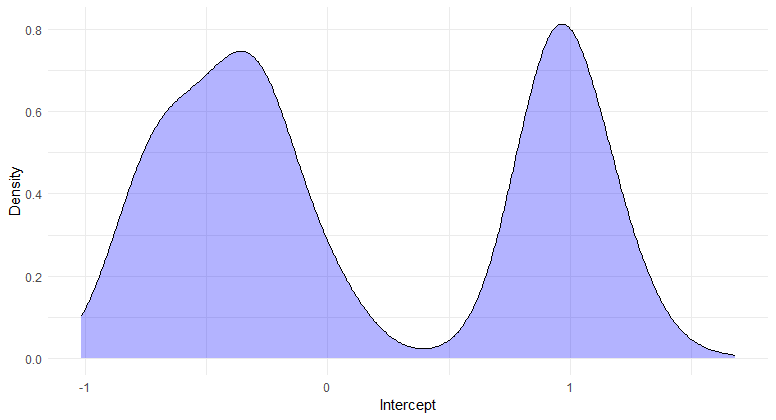
\includegraphics[width=340pt, height=200pt]{Chapters/chapter11/figures/DMPSemi.png}
	\caption[List of figure caption goes here]{Posterior density estimate: Mean of the stochastic errors.}\label{figDMPSemi}
\end{figure}

	\item \textbf{Example: Consumption of marijuana in Colombia continues II}

Perform the application of marijuana consumption with the following specification:
\begin{align*}
	y_i & = \boldsymbol{z}_i^{\top} \boldsymbol{\gamma} + f(Age_{i}) + \mu_i,
\end{align*}
where $y_i$ is the (log) marijuana monthly consumption, $\boldsymbol{z}_i$ represents the presence of a drug dealer in the neighborhood (\textit{Dealer}), gender (\textit{Female}), indicators of good physical and mental health (\textit{PhysicalHealthGood} and \textit{MentalHealthGood}), years of education (\textit{YearsEducation}), and the (log) prices of marijuana, cocaine, and crack by individual.

Initially, set the knots as the percentiles $\left\{0,0.05,\dots,0.95,1\right\}$ of age and use cubic B-splines. Then, apply the BIC approximation to perform variable selection in this model with non-informative conjugate priors, 5,000 MCMC iterations, and 5,000 burn-in iterations.

Do you think that using a linear regression with a second-degree polynomial in age provides a good approximation to the relationship found using splines in this application?

\textbf{Answer:}

The following code illustrates this exercise. We use the function \textit{bicreg} from the package \textit{BMA} to perform variable selection. Initially, we construct the design matrix, excluding the B-splines that cause perfect multicollinearity, and then select the variables with a posterior inclusion probability greater than 50\%. This also corresponds to the model with the highest posterior probability.

After this, we proceed with inference using a linear regression with conjugate prior distributions. Figure \ref{figAgeMarijuana} shows the fit, with the mean (blue line) and 95\% credible intervals (shaded blue). This curve is simpler than the one using all the B-splines: there appears to be a hook-shaped pattern at the beginning, where teenagers consume less marijuana than individuals in their 20s to 50s. After age 55, consumption decreases significantly. Given this pattern, assuming a second-degree polynomial appears to be a reasonable choice.

\begin{tcolorbox}[enhanced,width=4.67in,center upper,
	fontupper=\large\bfseries,drop shadow southwest,sharp corners]
	\textit{R code. Simulation: Semi-parametric Dirichlet process mixture}
	\begin{VF}
		\begin{lstlisting}[language=R]
rm(list = ls()); set.seed(010101) 
library(splines); library(ggplot2)
Data <- read.csv("https://raw.githubusercontent.com/BEsmarter-consultancy/BSTApp/refs/heads/master/DataApp/MarijuanaColombia.csv")
attach(Data)
IdOrd <- order(Age); y <- LogMarijuana[IdOrd]
Z <- as.matrix(cbind(Data[IdOrd,-c(1, 6, 7)]))
x <- Age[IdOrd] 
knots <- quantile(x, seq(0, 1, 0.05))
BS <- bs(x, knots = knots, degree = 3, Boundary.knots = range(x), intercept = FALSE)
matplot(x, BS, type = "l", lty = 1, col = rainbow(ncol(BS)))
# Function to check if a column is constant
is_constant <- function(col) {
	return(length(unique(col)) == 1)
}
constant_columns <- apply(BS, 2, is_constant)
X <- cbind(BS[,-c(which(constant_columns == TRUE))], Z)
BMAglm <- BMA::bicreg(X, y, strict = FALSE, OR = 50) 
summary(BMAglm)
idReg <- c(2, 23, 24, 27:29) # Relevant regressors, PIP > 0.5
Xnew <- cbind(1, X[, idReg])
N <- dim(Xnew)[1]; k <- dim(Xnew)[2]
# Hyperparameters
d0 <- 0.001; a0 <- 0.001
b0 <- rep(0, k); c0 <- 1000
B0 <- c0*diag(k); B0i <- solve(B0)
# MCMC parameters
mcmc <- 5000; burnin <- 5000
tot <- mcmc + burnin; thin <- 1
posterior  <- MCMCpack::MCMCregress(y~Xnew-1, b0=b0, B0 = B0i, c0 = a0, d0 = d0, burnin = burnin, mcmc = mcmc, thin = thin)
summary(coda::mcmc(posterior))
# Predict values with 95% credible intervals
xfit <- seq(min(x), max(x), 0.2); H <- length(xfit)
i <- 675 # Pick a particular individual
idfit <- sample(1:N, H)
BSfit <- bs(xfit, knots = knots, degree = 3, Boundary.knots = range(x), intercept = FALSE)
Xfit <- cbind(1, BSfit[,c(2,23)], Z[rep(i, H),c(1,4:6)]) # Relevant regressors, PIP > 0.5
Fit <- matrix(NA, mcmc, H)
for(s in 1:mcmc){
	Fit[s,] <- Xfit%*%posterior[s,1:7]
}
plot_data <- data.frame(x = xfit, fit = colMeans(Fit), liminf = apply(Fit, 2, quantile, 0.025), limsup = apply(Fit, 2, quantile, 0.975))

ggplot() + geom_line(data = plot_data, aes(x, fit), color = "blue", linewidth = 1) + geom_ribbon(data = plot_data, aes(x, ymin = liminf, ymax = limsup), fill = "blue", alpha = 0.2) + labs(title = "B-Spline Regression with 95% Confidence Interval", x = "Age",
y = "Log Marijuana") + theme_minimal()
\end{lstlisting}
	\end{VF}
\end{tcolorbox}

\begin{figure}[!h]
	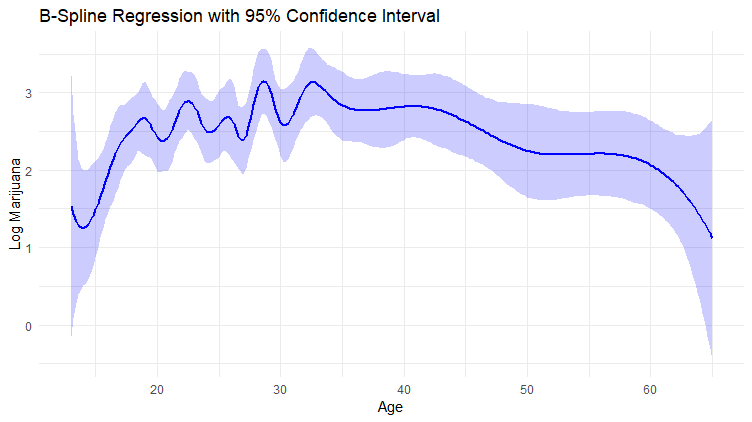
\includegraphics[width=340pt, height=200pt]{Chapters/chapter11/figures/AgeMarijuana.png}
	\caption[List of figure caption goes here]{Spline: Marijuana monthly consumption vs age.}\label{figAgeMarijuana}
\end{figure}

\end{enumerate}